\documentclass[11pt,psfig]{article}
\usepackage{epsfig}
\usepackage{times}
\usepackage{amssymb}
\usepackage{float}

\newcount\refno\refno=1
\def\ref{\the\refno \global\advance\refno by 1}
\def\ux{\underline{x}}
\def\uw{\underline{w}}
\def\bw{\underline{w}}
\def\ut{\underline{\theta}}
\def\umu{\underline{\mu}} 
\def\bmu{\underline{\mu}} 
\def\be{p_e^*}
\newcount\eqnumber\eqnumber=1
\def\eq{\the \eqnumber \global\advance\eqnumber by 1}
\def\eqs{\eq}
\def\eqn{\eqno(\eq)}

 \pagestyle{empty}
\def\baselinestretch{1.1}
\topmargin1in \headsep0.3in
\topmargin0in \oddsidemargin0in \textwidth6.5in \textheight8.5in
\begin{document}
\setlength{\parskip}{1.2ex plus0.3ex minus 0.3ex}


\thispagestyle{empty} \pagestyle{myheadings} \markright{Homework
1: CS 266, Computational Geometry: Spring 2014}



\title{CS 266 Homework 1}
\author{Zachary DeStefano, 15247592}
\date{Due Date: April 10, 2014}

\maketitle

\vfill\eject

\section*{Problem 1.6}

\subsection*{Problem 1.6 Part A}

Since the convex hull is a convex set containing all the points, it holds that the convex hull of the 2n endpoints is a convex set that contains all the line segments. Due to the convexity, all the line segments will be in the convex hull. 
\\
\\
Since the endpoints are on the line, a convex set of the n line segments must contain all the 2n endpoints. Since the convex hull of 2n endpoints is the smallest convex set that contains all the endpoints, it is thus the smallest convex set that contains all the n line segments, thus it is the convex hull of the line segments. 

\subsection*{Problem 1.6 Part B}

Let P be a non-convex polygon. Algorithm for finding the convex hull of P in O(n) time:
\\
1. Find left-most point and right-most point in polygon. 
2. To compute the upper hull, build up the line segments using the same algorithm as ConvexHull and use the vertices in lexicographic order of the polygon
3. Add or delete vertices depending on whether the slope is decreasing. 
TODO: Improve this description

\section*{Problem 1.10}

Let S be a set of n possibly intersecting unit circles

\subsection*{Problem 1.10a}

Proof that the convex hull of S consists of straight lines and pieces of circles in S. 
\\
A circle can be considered an infinite sided polygon. With this in mind, consider a set of regular k-gons with radius of 1. The convex hull will be convex set that contains all the vertices of the k-gons. There will thus be straight lines between each of the k-gons and parts of the hull be along the k-gon. 
\\
A circle is just a k-gon where $k=\infty$ thus the above holds for a circle. 

\subsection*{Problem 1.10b}

Assume that the convex hull appears on the boundary of a circle twice. There are two cases to consider.\\
Case 1: The convex hull is traveling along the circle and then goes inside the circle before going back to the boundary. \\
Case 2: The convex hull is traveling along the circle and then goes outside the circle before going back to the boundary.\\
\\
In case 1, you can connect the two end points and you will connect two points in the hull but part of the line will be outside the hull, thus it won't be a true convex hull, a contradiction\\
\\
In case 2, for the upper hull, the slope of the hull will have to increase to leave the hull. For the lower hull, the slope will have to decrease. This violates a basic constraint of convex hull, so we have a contradiction. \\
\\
Since we have a contradiction for both cases where a convex hull appears in two different places on the boundary of a circle, it is impossible for that to occur, thus the convex hull is either on the boundary once or not at all. 

\subsection*{Problem 1.10c}

Take the convex hull of S'. 
\\
Assume that a point is in the convex hull of S' but the corresponding circle is not on the boundary of the convex hull. This turns out to be a contradiction as there would be some other unaccounted for circle. \\
Assume that a circle is in the convex hull of S but its center is not in S', then there is some circle that was not considered and this eventually leads to a contradiction
\\
TODO: Improve the proof

\subsection*{Problem 1.10d}

The idea of the algorithm is that we will find the convex hull of the centers and then use that to get the total convex hull. Here is the algorithm:\\
1. Find the convex hull of the centers\\
2. For every line pq in that convex hull\\
			Find line perpendicular to pq that passes through p and line perpendicular to pq that passes through q, call them p1 and q1\\
			Find the interesection of the p circle with p1 and intersection of q circle with q1, call them p*, q*
			Connect p* and q* to be a line
3. The convex hull are all the straight lines and the circle boundaries between them

\subsection*{Problem 1.10e}

TODO: Figure out algorithm for hull if circles have different radii


\section*{Problem 8.2}

\subsection*{Problem 8.2a}

The dual of a collection of points inside a triangle with vertices p,q,r will be a collection of lines from the union of the double wedges for pq, qr, and pr. 
\\
When you take $p*, q*, r*$, the division of the plane forms 6 wedges. There are 7 faces when you include the inner triangle formed. In the following figure the dual ends up being everything except section 5 and 6. It will end up looking like a double wedge with an extra triangle in the middle. 

\begin{figure}[H]
\centering
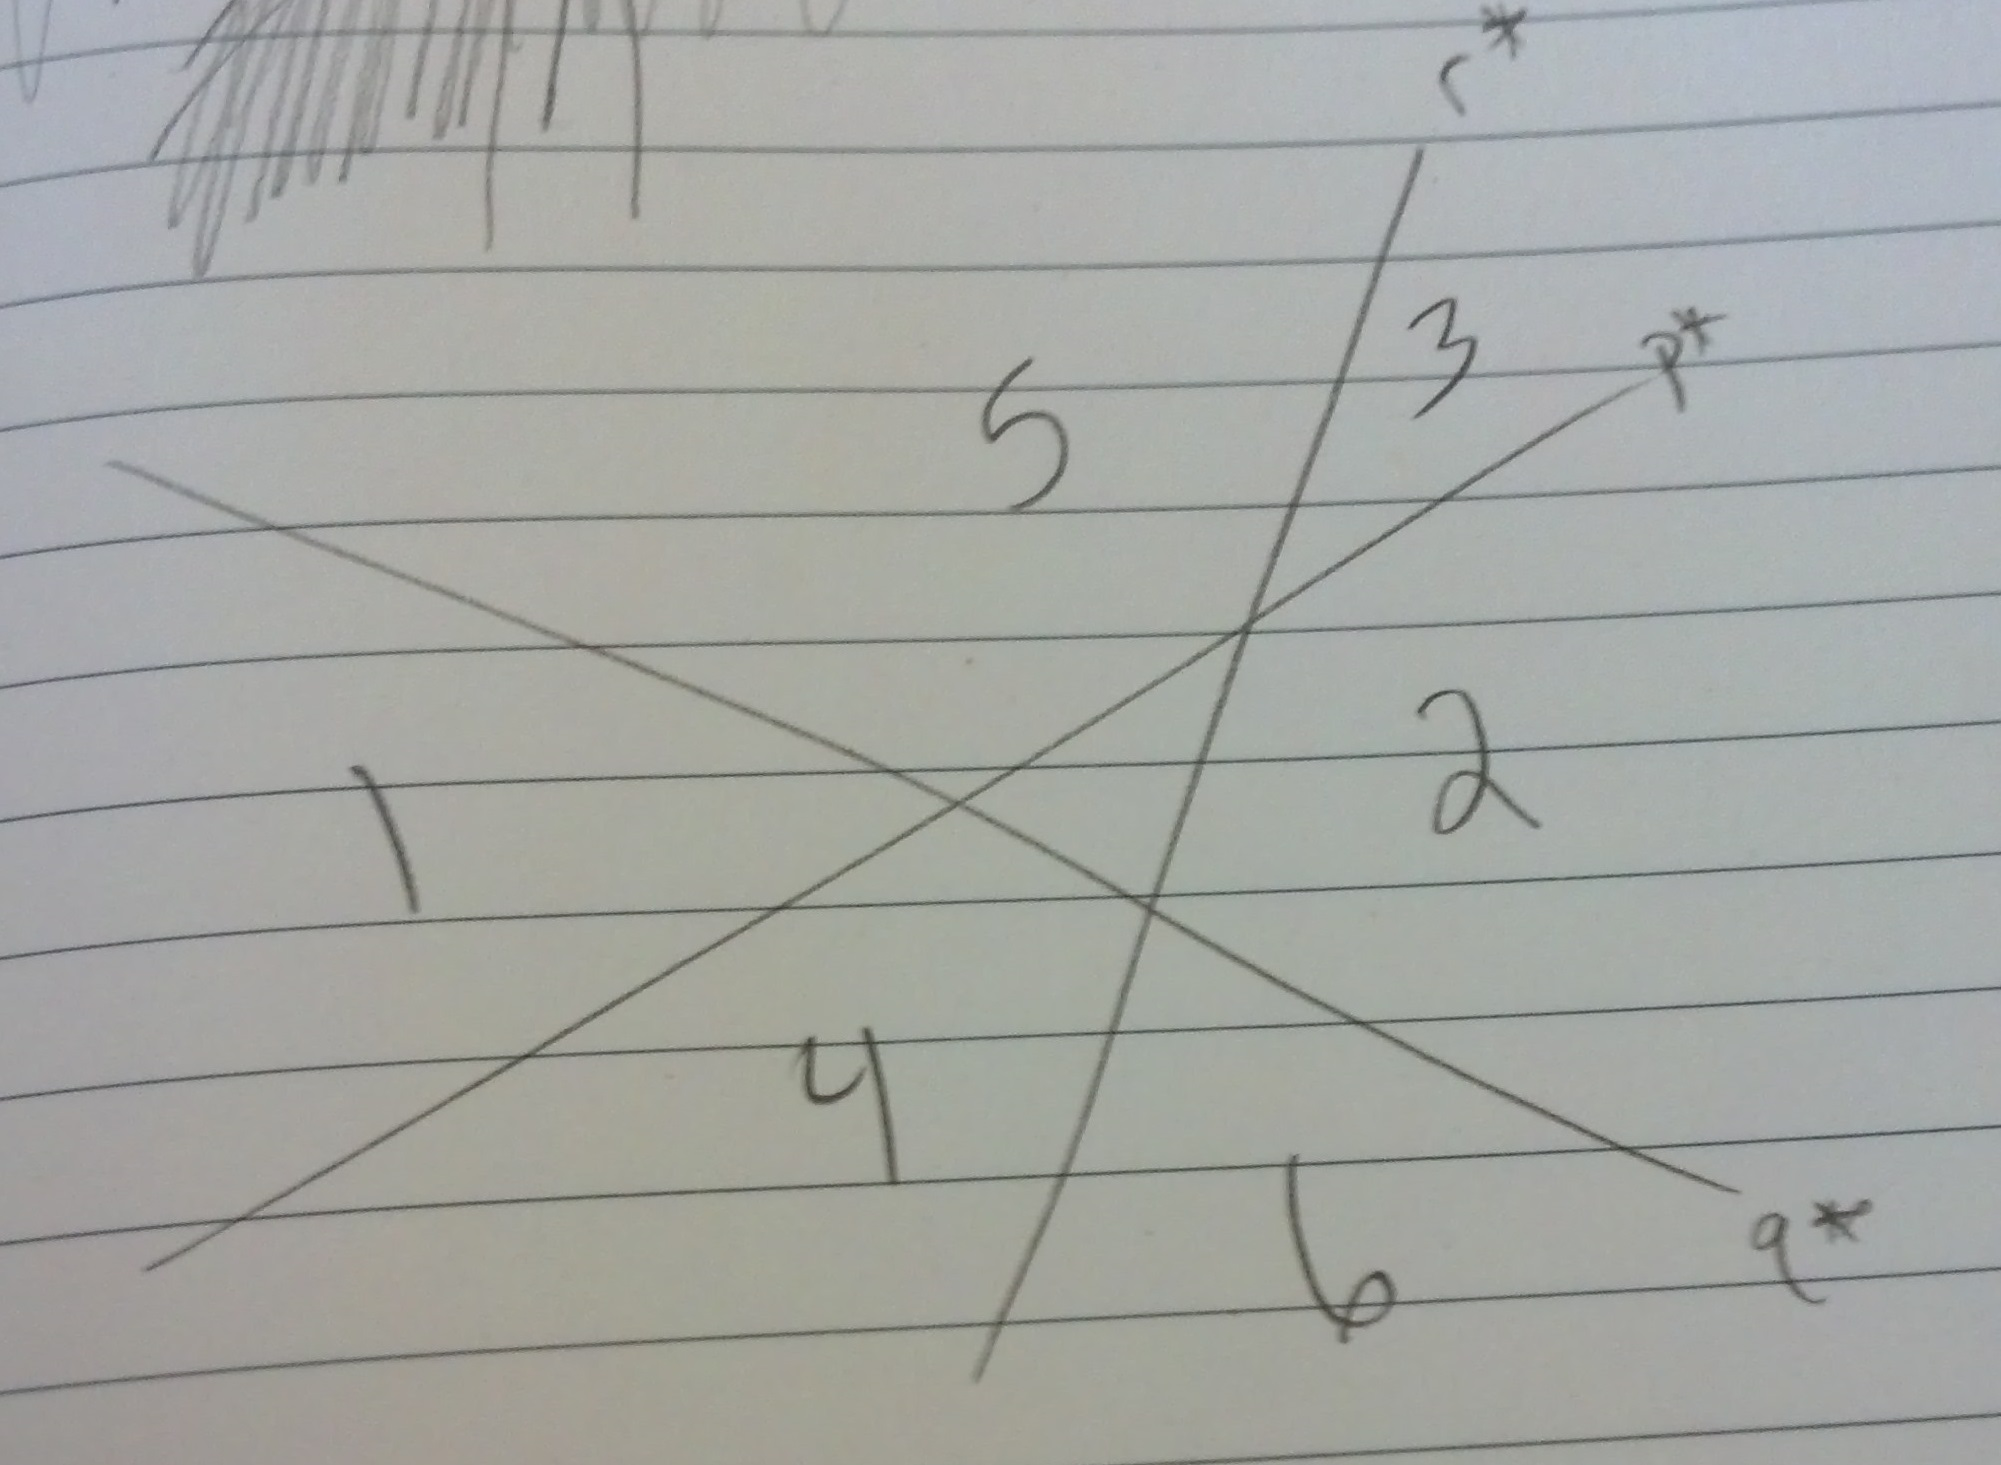
\includegraphics[height=4in]{cs266dual.jpg}
\caption{Illustration of the wedges}
\end{figure}

\subsection*{Problem 8.2b}

We will define a top-bottom double wedge in the following manner:
\\
- Take the intersection point of the double wedge $(x',y')$
\\
- Draw a horizontal line at that point, meaning the line $x=x'$. 
\\
- We have a top-bottom double wedge if one lies above that line and one lies below that line
\\
\\
The horizontal line has slope $0$ thus the wedge will cross that line if the slope goes from positive to negative. However, if the slope starts positive and increases or the slope starts negative and decreases, then it won't cross that line and will therefore be a top-bottom double wedge. 
\\
\\
Thus the following line segments have duals that are top-bottom double wedges:
- Line segments where both x-coordinates are positive and the slope is positive
- Line segments where both x-coordinates are negative and the slope is negative

\subsection*{Problem 8.2b Alternate}

In the illustration, the left-right double wedge is formed by the line segment. The dual lines all meet in that point since the primal points are co-linear. If we take the entire line formed by pq, the dual of that is the union of all lines that pass through that point. For the top-bottom double wedge, we want that whole union minus the left-right double wedge. \\
\\
Thus if you take the line $cx + d$ and take the points $p,q$ on it, then the two rays that are formed when you compute $(cx+d)-pq$ have a dual that is a top-bottom double wedge. 

\section*{Problem 8.6}

The duality transform is incidence-preserving thus the dual of the problem is whether any of the m points in the dual of L lie on any of the n lines in the dual of S. 


\end{document}








